\section{Preventivo}
Verranno utilizzate le seguenti abbreviazioni per indicare i ruoli:
\begin{itemize}
	\item \textbf{RE:} Responsabile;
	\item \textbf{AM:} Amministratore;
	\item \textbf{AN:} Analista;
	\item \textbf{PT:} Progettista;
	\item \textbf{PR:} Programmatore;
	\item \textbf{VE:} Verificatore.
\end{itemize}
Tenners applica le seguenti tariffe per tipo di ruolo coinvolto nell'attività di sviluppo:\\
\begin{table}[h]
\caption{Tabella tariffe per ruolo}            
\begin{center}
\begin{tabular}{ |c|c|  }
 \hline
 Ruolo 		& Tariffa (EUR)\\
 \hline\hline
	Responsabile	& 30\\
	Amministratore	& 20\\
	Analista		& 25\\
	Progettista		& 22\\
	Programmatore	& 15\\
	Verificatore	& 15\\
 \hline
\end{tabular}
\end{center}
\end{table}
\newpage
\subsection{Analisi dei requisiti}
\subsubsection{Prospetto orario}
Il team ha previsto la seguente suddivisione di ruoli durante questo periodo:\\
\begin{table}[h]
\caption{Tabella suddivisione per ruolo, Analisi dei requisiti}  
\begin{center}
\begin{tabular}{ |c|c|c|c|c|c|c|c|  }
 \hline
 Membro 		& RE 	& AM 	& AN 	& PT 	& PR 	& VE 	& Tot.\\
 \hline\hline
 Simone	Franconetti		& 4 		& 4 		& 14 	& 2 		& 0 		& 6 		& 30\\
 Gabriel Ciulei			& 3 		& 2 		& 20 	& 2 		& 0 		& 3 		& 30\\
 Nicola	Salvadore		& 6 		& 4 		& 10 	& 0 		& 0 		& 10 	& 30\\
 Gianmarco	Pettinato	& 0 		& 2 		& 16 	& 2 		& 0 		& 10 	& 30\\
 Gezim	Cikaqi			& 6 		& 10 	 	& 6 		& 2 		& 0 		& 6	 	& 30\\
 Paola	Trevisan		& 6 		& 2 		& 10 	& 2 		& 0 		& 10 	& 30\\
 Giovanni	Incalza		& 6 		& 11 		& 8 		& 0 		& 0 		& 5  	& 30\\
 \hline\hline
 Ore totali		& 31		& 35		& 84 	& 10 	& 0 		& 50 	& 210\\
  \hline
\end{tabular}
\end{center}
\end{table}
\begin{figure}[h!]
	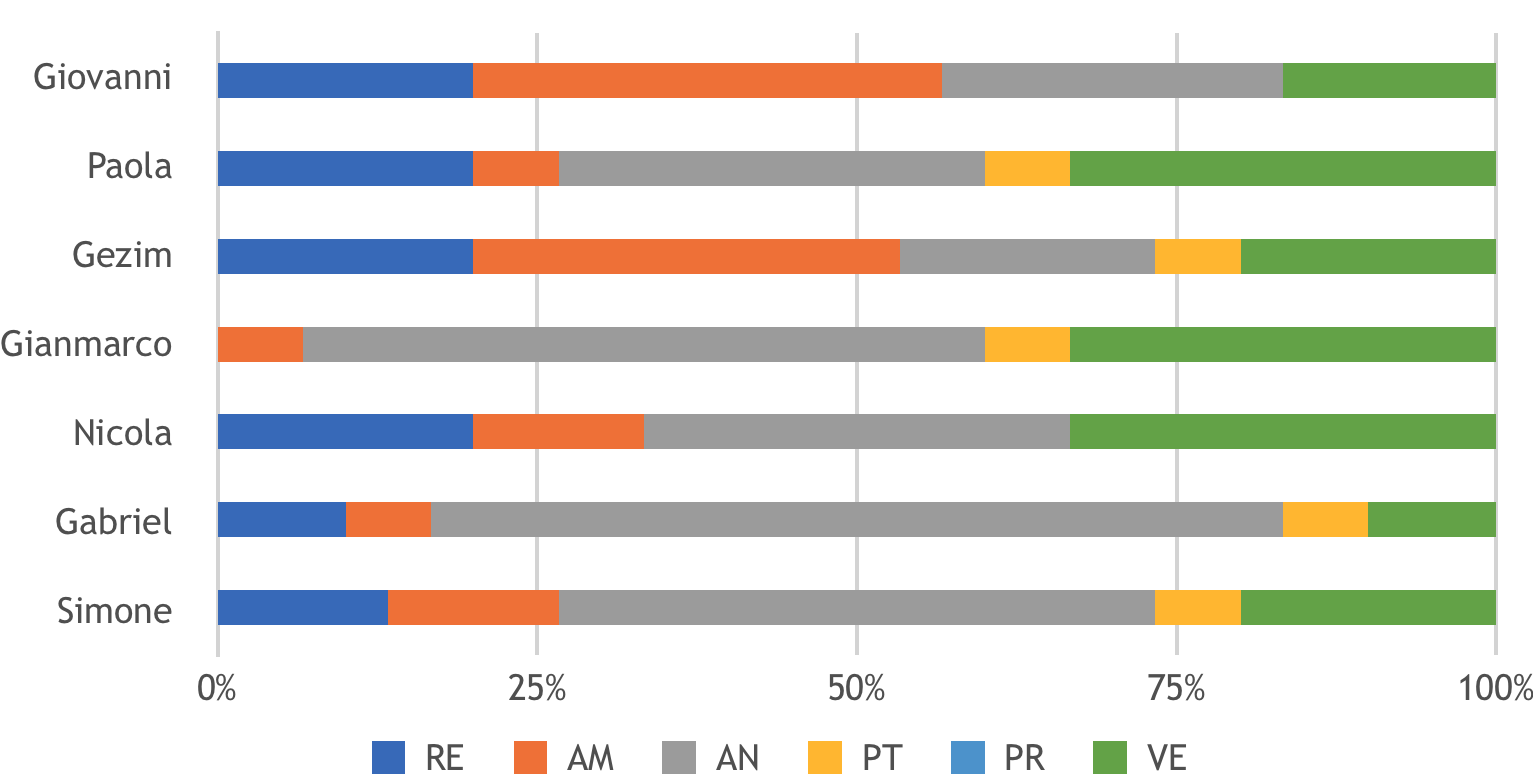
\includegraphics[width=\textwidth]{res/img/hi17}
	\caption{Diagramma della suddivisione dei ruoli, Analisi dei requisiti}
\end{figure}

\subsubsection{Prospetto economico}
In base alle ore necessarie per il completamento di questa fase, il valore economico totale è di 4.700,00 EUR.
\begin{table}[h]
	\caption{Tabella prospetto economico, Analisi dei requisiti}  
\begin{center}
\begin{tabular}{ |c|c|c|  }
 \hline
 Ruolo 		& Ammontare ore 	& Totale (EUR)\\
 	\hline
 \hline
 	Responsabile	& 31 	& 930\\
	Amministratore	& 35		& 700\\
	Analista		& 84 	& 2100\\
	Progettista		& 10		& 220\\
	Programmatore	& 0		& 0\\
	Verificatore	& 50		& 750\\
 \hline\hline
 TOTALE		& 210		& 4700\\
  \hline
\end{tabular}
\end{center}
\end{table}
\newpage
\subsection{Progettazione architetturale}
\subsubsection{Prospetto orario}
Il team ha previsto la seguente suddivisione di ruoli per questa fase del progetto:
\\
\begin{table}[h]
\caption{Tabella suddivisione per ruolo, Progettazione architetturale}  
\begin{center}
\begin{tabular}{ |c|c|c|c|c|c|c|c|  }
 \hline
 Membro 		& RE 	& AM 	& AN 	& PT 	& PR 	& VE 	& Tot.\\
 \hline\hline
 Simone	Franconetti		& 5 		& 0		& 6 	& 13 	& 6 		& 0 		& 30\\
 Gabriel Ciulei		& 0 		& 5 		& 2 	& 15		& 8 		& 0 		& 30\\
 Nicola	Salvadore		& 0 		& 2 		& 4 	& 8		& 8 		& 8 		& 30\\
 Gianmarco	Pettinato	& 5 		& 8 		& 3 	& 10 	& 2 		& 2 		& 30\\
 Gezim	Cikaqi		& 0 		& 0 		& 10 	& 10		& 4 		& 6	 	& 30\\
 Paola	Trevisan		& 0 		& 4 		& 6 	& 8 		& 6 		& 6 		& 30\\
 Giovanni Incalza		& 0 		& 0	 	& 8 	& 10		& 4 		& 8  	& 30\\
 \hline\hline
 Ore totali		& 10		& 19		& 39 	& 74	 	& 38 	& 30 	& 210\\
  \hline
\end{tabular}
\end{center}
\end{table}
\begin{figure}[h!]
	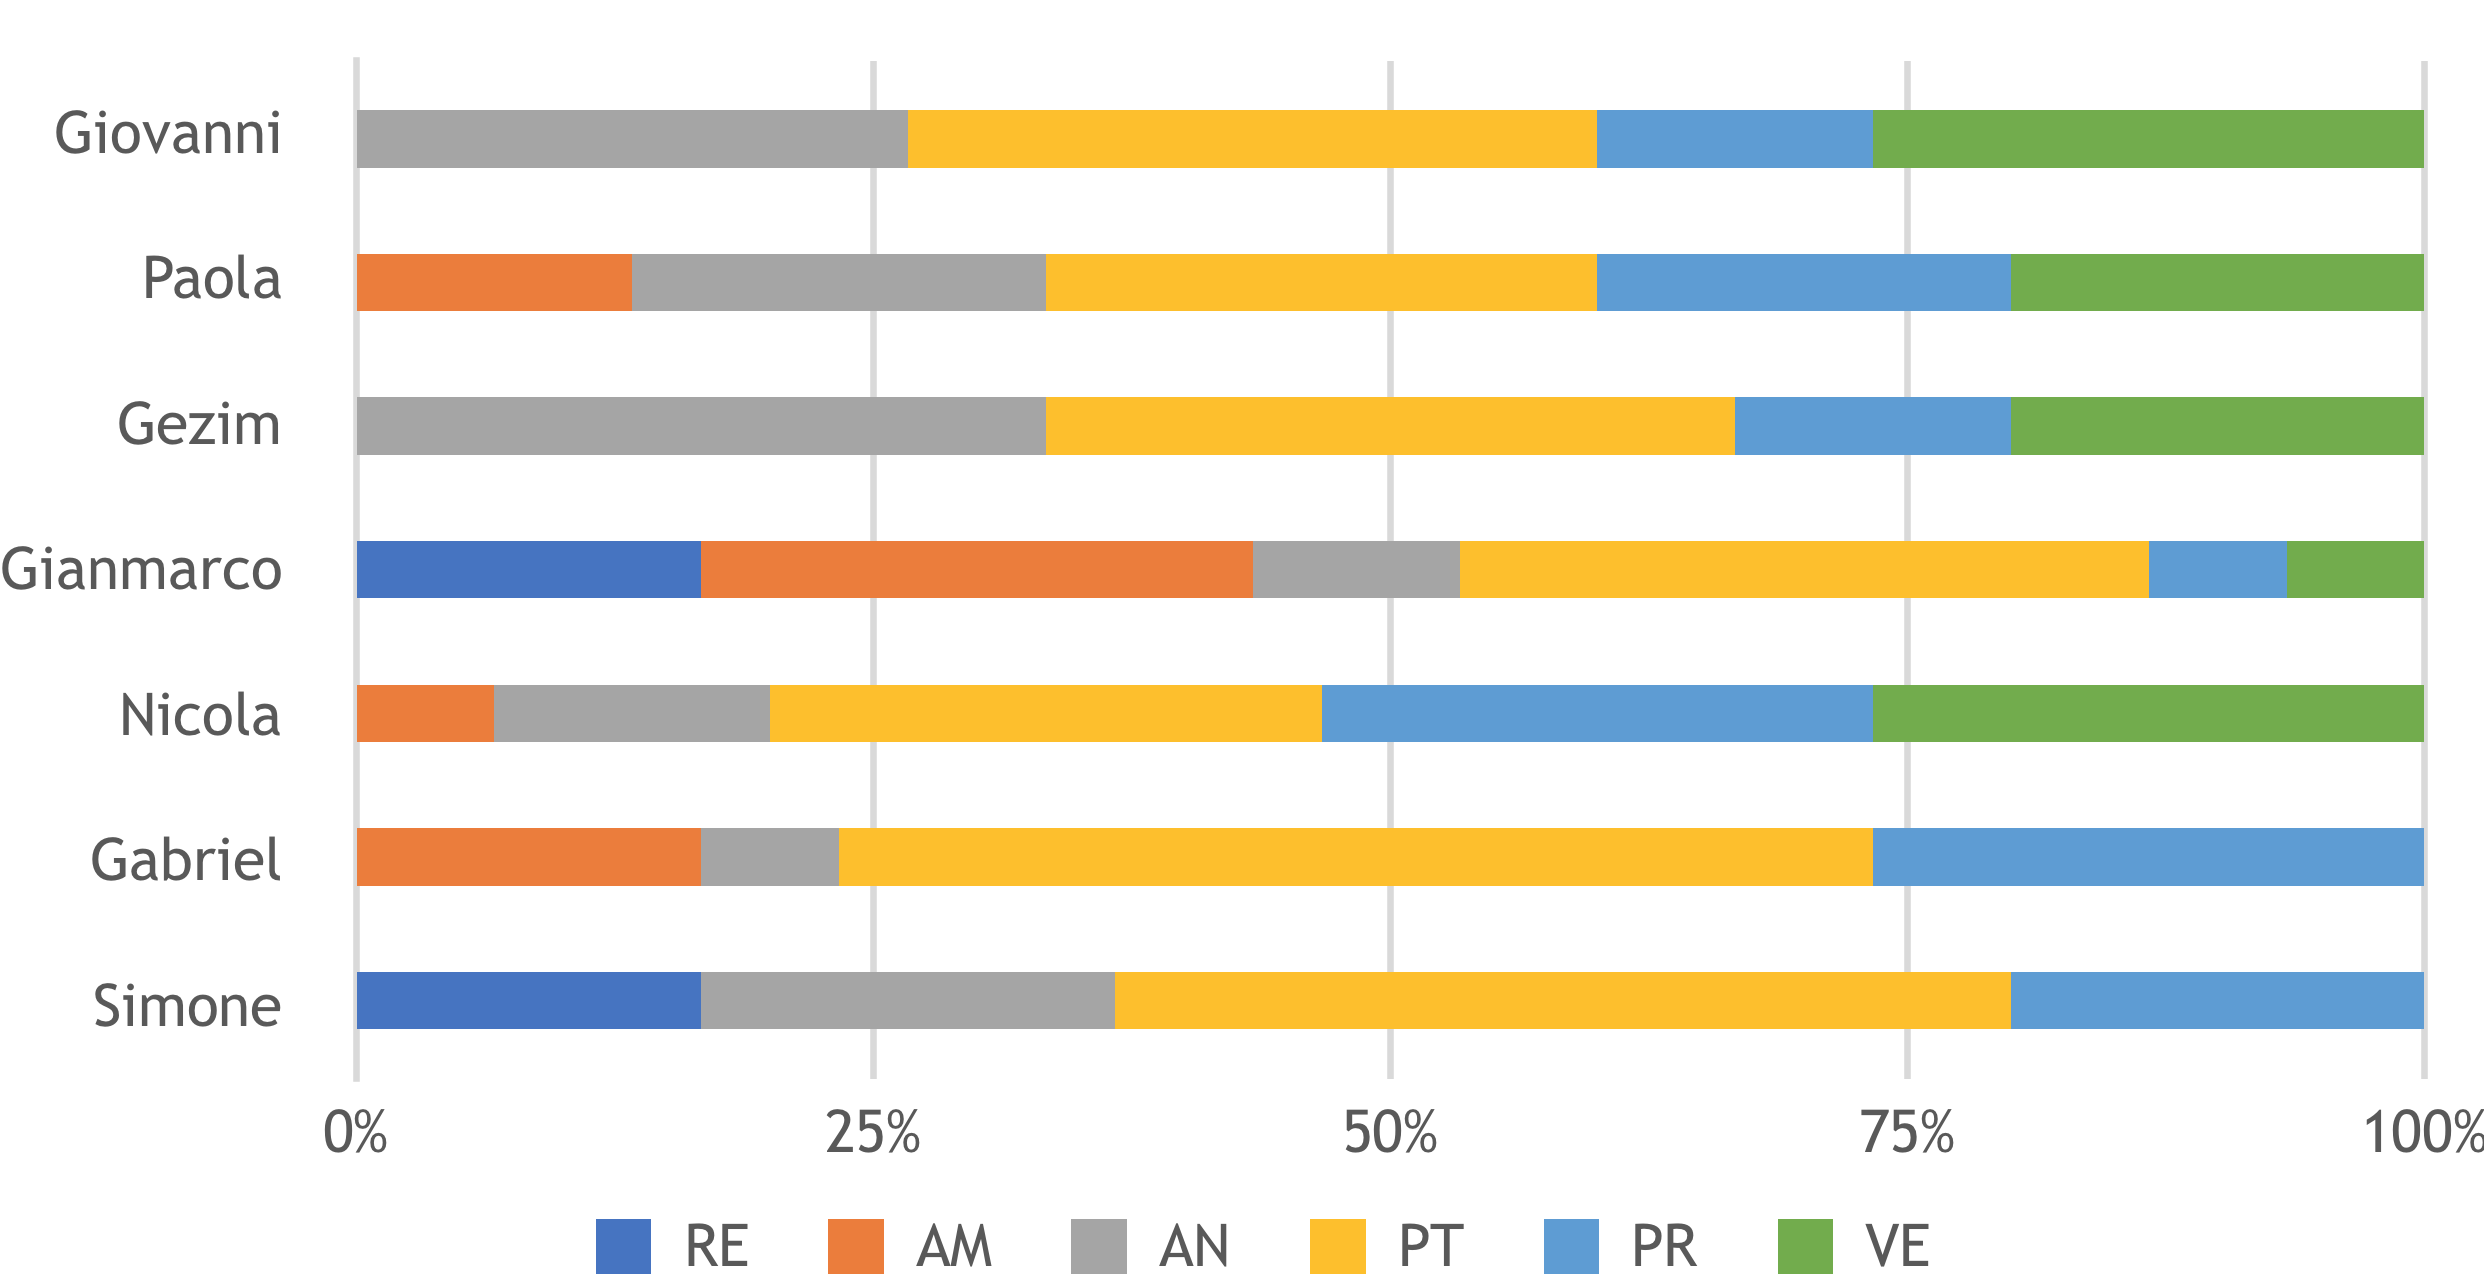
\includegraphics[width=\textwidth]{res/img/hi336}
	\caption{Diagramma della suddivisione dei ruoli, Progettazione architetturale}
\end{figure}

\subsubsection{Prospetto economico}
In base alle ore necessarie per il completamento di questa fase, il valore economico totale è di 4.303,00 EUR.
\begin{table}[h]
	\caption{Tabella prospetto economico, Progettazione architetturale}  
\begin{center}
\begin{tabular}{ |c|c|c|  }
 \hline
 Ruolo 		& Ammontare ore 	& Totale (EUR)\\
 	\hline
 \hline
 	Responsabile	& 10 	& 300\\
	Amministratore	& 19		& 380\\
	Analista		& 39 	& 975\\
	Progettista		& 74		& 1628\\
	Programmatore	& 38		& 570\\
	Verificatore	& 30 	& 450\\
 \hline\hline
 TOTALE		& 210		& 4303\\
  \hline
\end{tabular}
\end{center}
\end{table}
\newpage
\subsection{Progettazione di dettaglio e codifica}
\subsubsection{Prospetto orario}
Il team ha previsto la seguente suddivisione di ruoli per questa fase del progetto:
\begin{table}[h]
\caption{Tabella suddivisione per ruolo, Progettazione di dettaglio e codifica}  
\begin{center}
\begin{tabular}{ |c|c|c|c|c|c|c|c|  }
 \hline
 Membro 		& RE 	& AM 	& AN 	& PT 	& PR 	& VE 	& Tot.\\
 \hline\hline
 Simone	Franconetti		& 0 		& 8		& 2 	& 10 	& 25 		& 10 		& 55\\
 Gabriel Ciulei		& 5 		& 0 		& 0 	& 10		& 30 		& 10 		& 55\\
 Nicola	Salvadore		& 5 		& 8 		& 3 	& 9 		& 20 		& 10 		& 55\\
 Gianmarco	Pettinato	& 0 		& 0 		& 0 	& 15 	& 30 		& 10 		& 55\\
 Gezim	Cikaqi		& 5 		& 6 		& 0 	& 12 	& 24 		& 8	 		& 55\\
 Paola	Trevisan		& 5 		& 2 		& 3 	& 15 	& 20 		& 10 		& 55\\
 Giovanni	Incalza	& 5 		& 6	 	& 0 	& 10 	& 24 		& 10  		& 55\\
 \hline\hline
 Ore totali		& 25		& 30		& 8 	& 81	 	& 173 	& 68 	& 385\\
  \hline
\end{tabular}
\end{center}
\end{table}
\begin{figure}[h!]
	\centering
	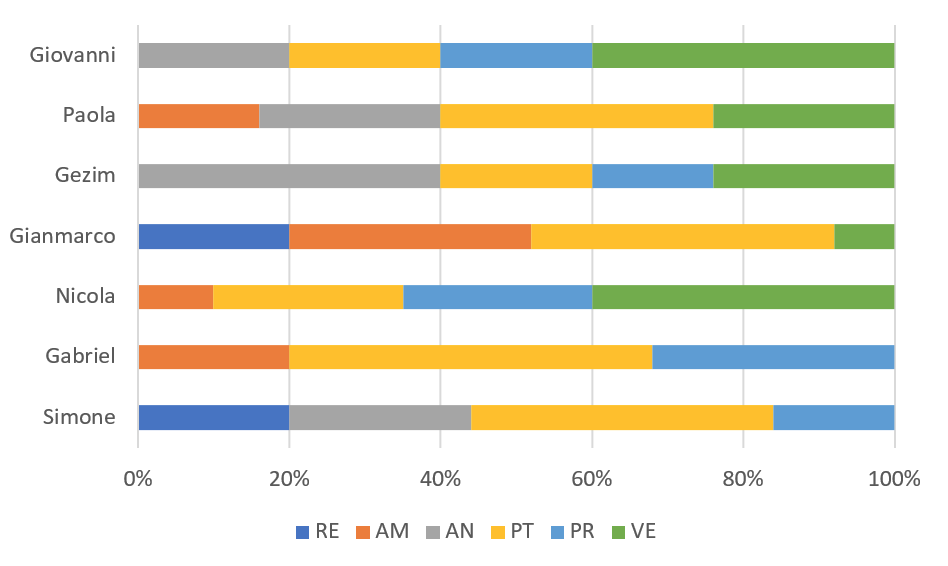
\includegraphics[width=0.9\textwidth]{res/img/hi33}
	\caption{Diagramma della suddivisione dei ruoli, Progettazione di dettaglio e codifica}
\end{figure}

\subsubsection{Prospetto economico}
In base alle ore necessarie per il completamento di questa fase, il valore economico totale è di 6.947,00 EUR.
\begin{table}[h]
\caption{Tabella prospetto economico, Progettazione di dettaglio e codifica}  
\begin{center}
\begin{tabular}{ |c|c|c|  }
 \hline
 Ruolo 		& Ammontare ore 	& Totale (EUR)\\
 	\hline
 \hline
 	Responsabile	& 25 		& 750\\
	Amministratore	& 30		& 600\\
	Analista		& 8 	& 200\\
	Progettista		& 81		& 1782\\
	Programmatore	& 173		&2595 \\
	Verificatore	& 68 	& 1020\\
 \hline\hline
 TOTALE		& 385		& 6947\\
  \hline
\end{tabular}
\end{center}
\end{table}
\newpage
\subsection{Validazione e Collaudo}
\subsubsection{Prospetto orario}
Il team ha previsto la seguente suddivisione di ruoli per questa fase del progetto:
\begin{table}[h]
\caption{Tabella suddivisione per ruolo, Validazione e Collaudo}  
\begin{center}
\begin{tabular}{ |c|c|c|c|c|c|c|c|  }
 \hline
 Membro 		& RE 	& AM 	& AN 	& PT 	& PR 	& VE 	& Tot.\\
 \hline\hline
 Simone Franconetti			& 4 		& 0		& 0 	& 2 		& 4 		& 10 		& 20\\
 Gabriel Ciulei		& 0 		& 6 		& 0 	& 4		& 2 		& 8 		& 20\\
 Nicola	Salvadore		& 0 		& 0 		& 0 	& 6 		& 4 		& 10 		& 20\\
 Gianmarco Pettinato		& 4 		& 6 		& 0 	& 0	 	& 4 		& 6 		& 20\\
 Gezim Cikaqi			& 0 		& 2 		& 0 	& 0 		& 8 		& 10	 	& 20\\
 Paola Trevisan			& 4 		& 4 		& 0 	& 0 		& 8 		& 4 		& 20\\
 Giovanni Incalza		& 2 		& 0	 	& 0 	& 2 		& 12 	& 4  	& 20\\
 \hline\hline
 Ore totali		& 14		& 18		& 0 	& 14	 	& 42 	& 52 	& 140\\
  \hline
\end{tabular}
\end{center}
\end{table}
\begin{figure}[h!]
	\centering
	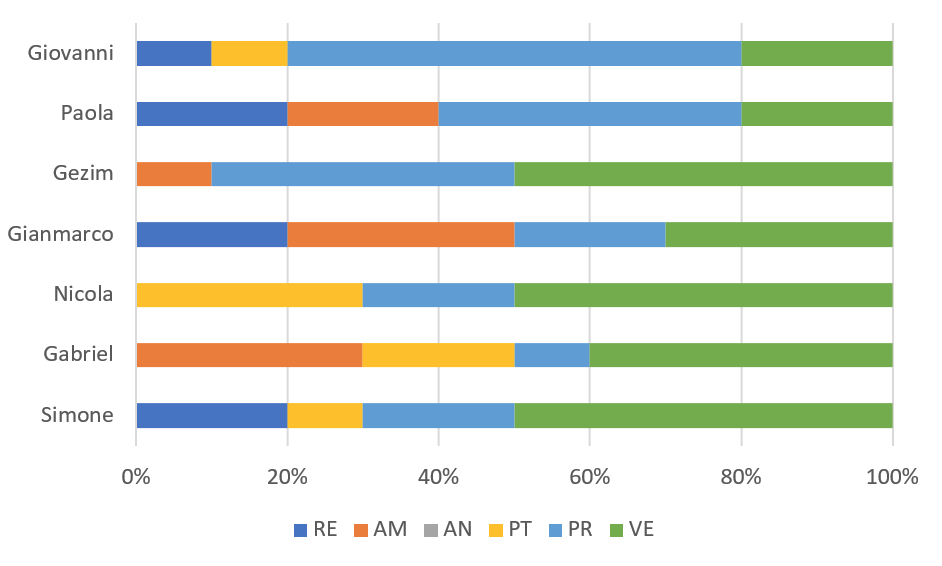
\includegraphics[width=0.9\textwidth]{res/img/hi5}
	\caption{Diagramma della suddivisione dei ruoli, Validazione e Collaudo}
\end{figure}

\subsubsection{Prospetto economico}
In base alle ore necessarie per il completamento di questa fase, il valore economico totale è di 2.498,00 EUR.
\begin{table}[h]
\caption{Tabella prospetto economico, Verifica e Collaudo}  
\begin{center}
\begin{tabular}{ |c|c|c|  }
 \hline
 Ruolo 		& Ammontare ore 	& Totale (EUR)\\
 \hline
 \hline
 	Responsabile	& 14 	& 420\\
	Amministratore	& 18		& 360\\
	Analista		& 0 		& 0\\
	Progettista		& 14		& 308\\
	Programmatore	& 42		& 630\\
	Verificatore	& 52 	& 780\\
 \hline\hline
 TOTALE		& 140		& 2498\\
  \hline
\end{tabular}
\end{center}
\end{table}
\newpage
\subsection{Riepilogo}
\subsubsection{Prospetto orario}
Il team ha previsto la seguente suddivisione di ruoli per il completamento del progetto:
\begin{table}[h]
\caption{Tabella di riepilogo del prospetto orario}  
\begin{center}
\begin{tabular}{ |c|c|c|c|c|c|c|c|  }
 \hline
 Membro 		& RE 		& AM 		& AN 	& PT 	& PR 	& VE 	& Tot.\\
 \hline\hline
 Simone	Franconetti		& 13 		& 16			& 23 		& 24 		& 33 		& 26 		& 140\\
 Gabriel Ciulei		& 8 			& 13 		& 22 		& 28		& 40 		& 24 		& 140\\
 Nicola	Salvadore		& 11 		& 14 		& 16 		& 22 		& 32 		& 40 		& 140\\
 Gianmarco Pettinato		& 12 		& 16 		& 18 		& 27	 	& 34 		& 28 		& 140\\
 Gezim Cikaqi		& 11 		& 18 		& 18 		& 19 		& 36 		& 33	 	& 140\\
 Paola Trevisan		& 15 		& 12 		& 24 		& 26 		& 28 		& 30 		& 140\\
 Giovanni	Incalza	& 13 		& 17	 		& 16 		& 17 		& 41	 	& 31  		& 140\\
 \hline\hline
 Ore totali		& 83 	& 106		& 149 	& 179 	& 253 	& 210 	& 980\\
  \hline
\end{tabular}
\end{center}
\end{table}
\begin{figure}[h!]
	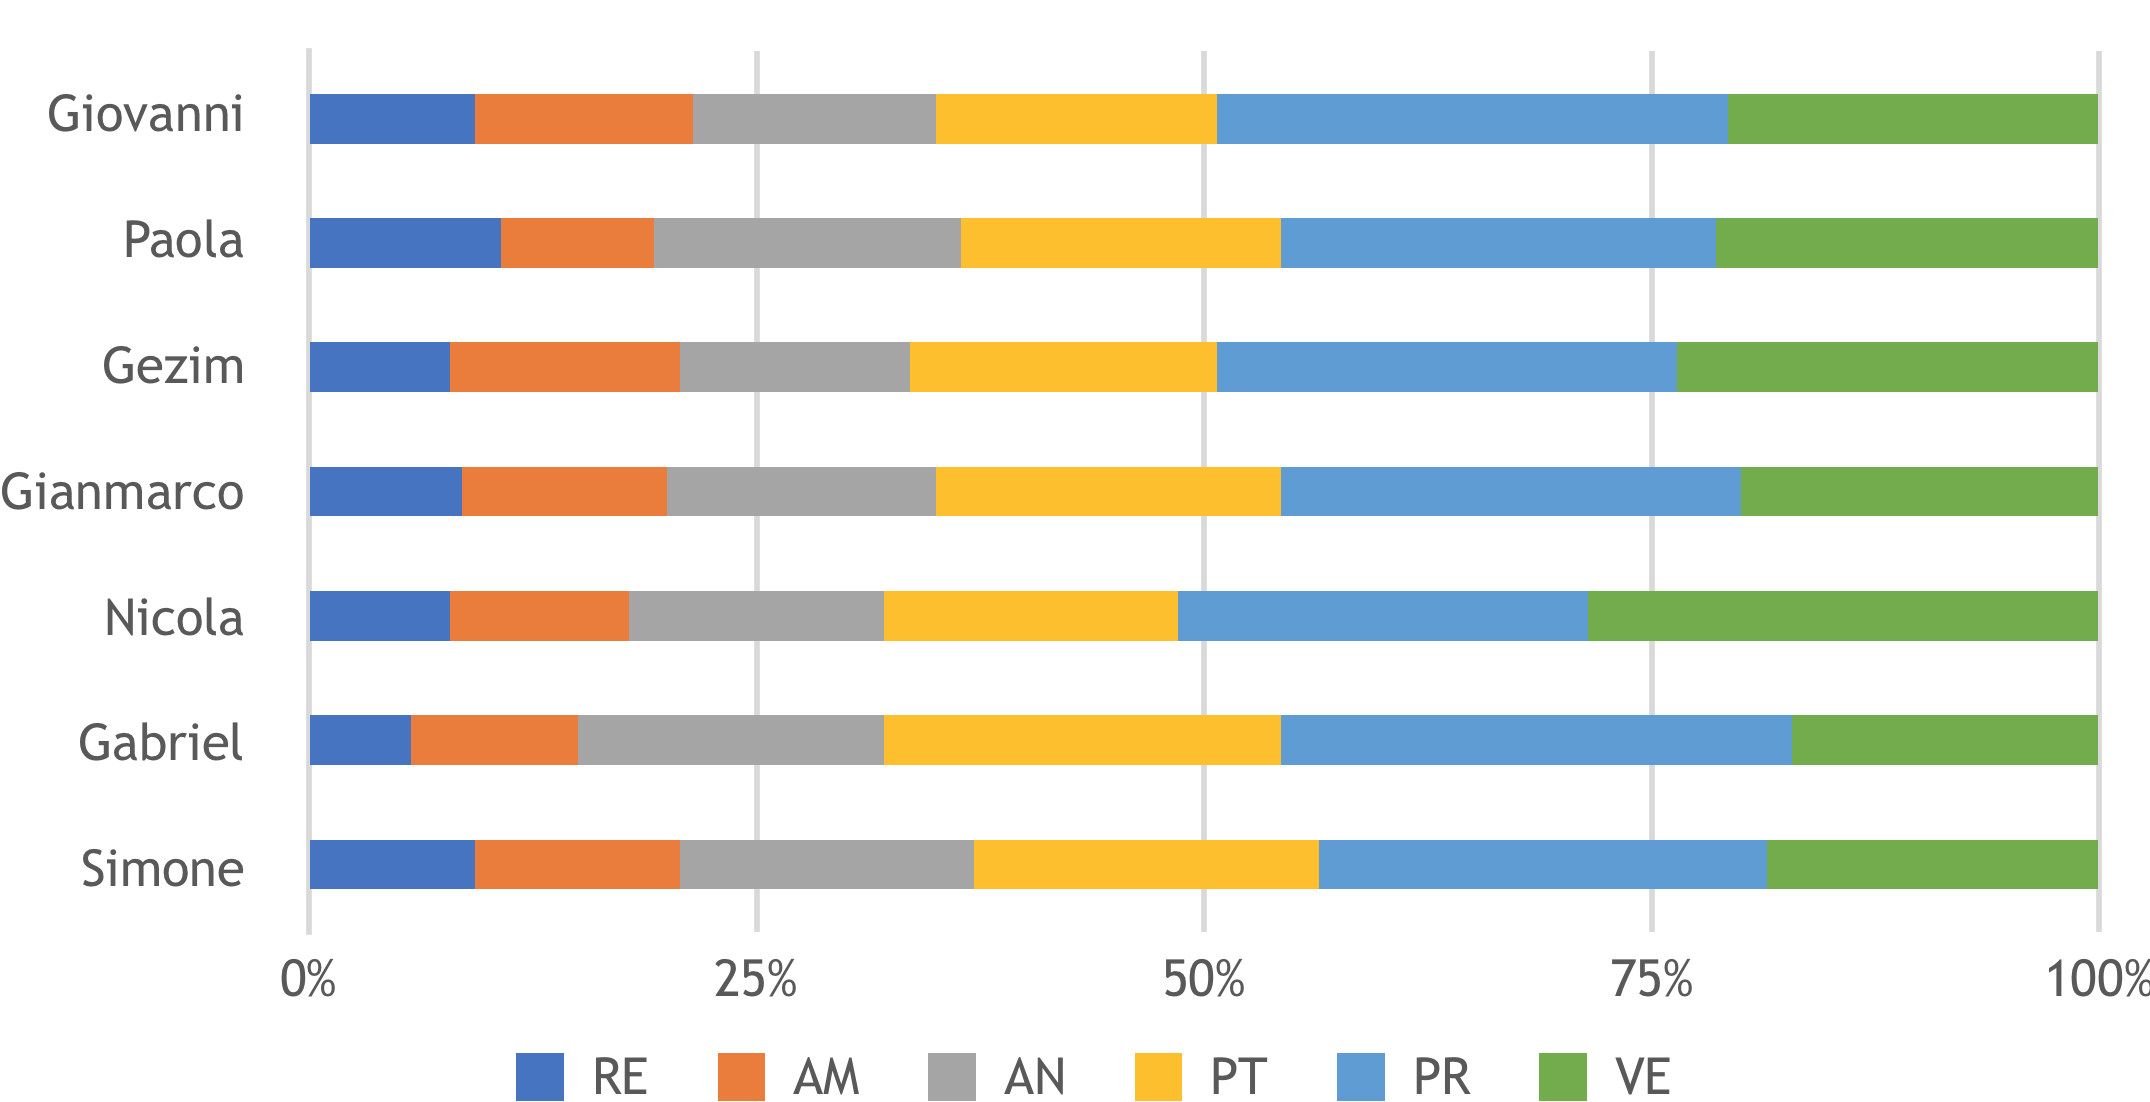
\includegraphics[width=\textwidth]{res/img/hip3}
	\caption{Diagramma della suddivisione dei ruoli durante l'intero il progetto}
\end{figure}

\subsubsection{Prospetto economico}
In base alle ore necessarie per il completamento di questo progetto, il valore economico totale è di 19.218,00 EUR.
\begin{table}[h]
\caption{Tabella di riepilogo del prospetto economico}  
\begin{center}
\begin{tabular}{ |c|c|c|  }
 \hline
 Ruolo 		& Ammontare ore 	& Totale (EUR)\\
 \hline
 \hline
 	Responsabile	& 83 		& 2490\\
	Amministratore	& 106		& 2120\\
	Analista		& 149 		& 3725\\
	Progettista		& 179		& 3938\\
	Programmatore	& 253		& 3795\\
	Verificatore	& 210 		& 3150\\
 \hline\hline
 TOTALE		& 980		& 19218\\
  \hline
\end{tabular}
\end{center}
\end{table}

\subsubsection{Conclusioni}
Il valore economico del progetto è di 19.218,00 EUR. Tuttavia a questo totale bisogna sottrarre il corrispettivo delle fasi Analisi (4.700,00 EUR) e Presentazione (770,00 EUR) in quanto tali fasi non producono valore per il committente.
\newline
\newline
In conclusione, il totale preventivato per la realizzazione del progetto \textit{Etherless} è di\\ \textbf{13.748,00 EUR}, valore che rispecchia il numero di ore rendicontabili per ogni figura professionale che verrà coinvolta durante la realizzazione del progetto. 
\begin{table}[h]
\caption{Tabella di riepilogo del prospetto economico (escluso il periodo iniziale di \textit{Analisi dei requisiti})} 
\begin{center}
\begin{tabular}{ |c|c|c|  }
 \hline
 Ruolo 		& Ammontare ore 	& Totale (EUR)\\
 \hline
 \hline
 	Responsabile	& 49 	& 1470\\
	Amministratore	& 67		& 1340\\
	Analista		& 47 	& 1175\\
	Progettista		& 169	& 3718\\
	Programmatore	& 253	& 3795\\
	Verificatore	& 150 	& 2250\\
 \hline\hline
 TOTALE		& 735		& 13748\\
  \hline
\end{tabular}
\end{center}
\end{table}
Nello specifico, la programmazione della suddivisione del lavora prevede la seguente divisione dei ruoli per i singoli membri del team:
\begin{table}[h]
	\caption{Tabella di riepilogo del prospetto orario (escluso il periodo iniziale di \textit{Analisi dei requisiti})} 
\begin{center}
\begin{tabular}{ |c|c|c|c|c|c|c|c|  }
 \hline
 Membro 		& RE 		& AM 		& AN 	& PT 	& PR 	& VE 	& Tot.\\
 \hline\hline
 Simone	Franconetti		& 9  	 	& 8			& 2 		& 25 		& 35 		& 20 		& 105\\
 Gabriel Ciulei		& 5 			& 11 		& 2 		& 29			& 40 		& 18 		& 105\\
 Nicola	Salvadore		& 5  		& 10 		& 7 		& 23 		& 32 		& 28 		& 105\\
 Gianmarco	Pettinato	& 9   		& 14 		& 3 		& 25		 	& 36 		& 18 		& 105\\
 Gezim	Cikaqi		& 5  		& 8  		& 10		& 22 		& 36 		& 24	 	& 105\\
 Paola	Trevisan		& 9  		& 10 		& 9 		& 23 		& 34 		& 20 		& 105\\
 Giovanni	Incalza	& 7  		& 6	 		& 8 		& 22 		& 40		 	& 22  		& 105\\
 \hline\hline
 Ore totali		& 49 	& 67		& 47 	& 169 	& 253 	& 150 	& 735\\
  \hline
\end{tabular}
\end{center}
\end{table}
